
\begin{figure}
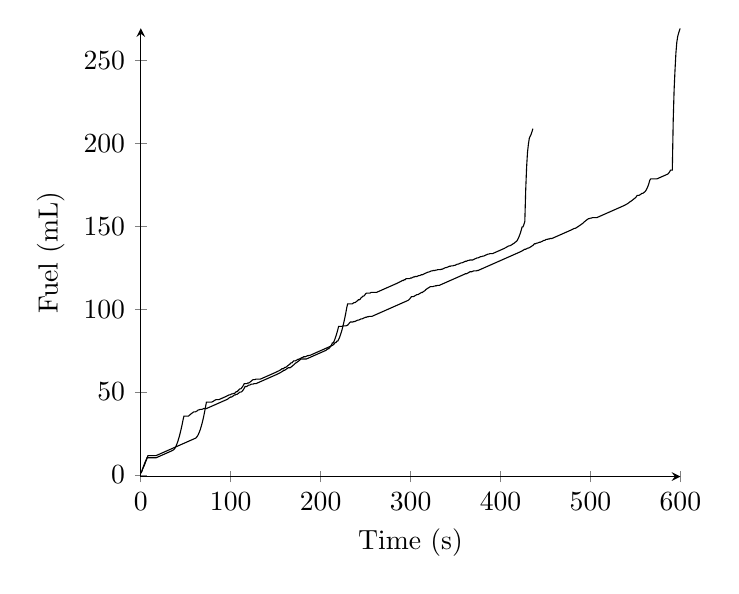
\begin{tikzpicture}
\begin{axis}[
legend style={anchor=west},
axis x line=bottom,
axis y line=left,
ymin=-1,
xlabel=Time (s),
ylabel=Fuel (mL),
]
\addplot[] coordinates {
(0, 1.00398986302)
(1, 1.97828846122)
(2, 3.34660470616)
(3, 5.13437979035)
(4, 6.52790829324)
(5, 7.93992034887)
(6, 9.04639231824)
(7, 10.2564622455)
(8, 11.6265487206)
(9, 11.6265487206)
(10, 11.6265487206)
(11, 11.6265487206)
(12, 11.6265487206)
(13, 11.6265487206)
(14, 11.6265487206)
(15, 11.6265487206)
(16, 11.6265487206)
(17, 11.6265487206)
(18, 11.8664342339)
(19, 12.1063197473)
(20, 12.3462052607)
(21, 12.586090774)
(22, 12.8259762874)
(23, 13.0658618007)
(24, 13.3057473141)
(25, 13.5456328275)
(26, 13.7855183408)
(27, 14.0254038542)
(28, 14.2652893675)
(29, 14.5051748809)
(30, 14.7450603943)
(31, 14.9849459076)
(32, 15.224831421)
(33, 15.4647169344)
(34, 15.7046024477)
(35, 15.9444879611)
(36, 16.1843734744)
(37, 16.4242589878)
(38, 16.6641445012)
(39, 16.9040300145)
(40, 17.1439155279)
(41, 17.3838010412)
(42, 17.6236865546)
(43, 17.863572068)
(44, 18.1034575813)
(45, 18.3433430947)
(46, 18.5832286081)
(47, 18.8231141214)
(48, 19.0629996348)
(49, 19.3028851481)
(50, 19.5427706615)
(51, 19.7826561749)
(52, 20.0225416882)
(53, 20.2624272016)
(54, 20.5023127149)
(55, 20.7421982283)
(56, 20.9820837417)
(57, 21.221969255)
(58, 21.4618547684)
(59, 21.7017402818)
(60, 21.9416257951)
(61, 22.1815113085)
(62, 22.6918940297)
(63, 23.4152575652)
(64, 24.4306091641)
(65, 25.6352162014)
(66, 27.1230102966)
(67, 28.8422678614)
(68, 30.8083209851)
(69, 32.9527073872)
(70, 35.3939277451)
(71, 38.0955415998)
(72, 40.9859538409)
(73, 43.9453199331)
(74, 43.9453199331)
(75, 43.9453199331)
(76, 43.9453199331)
(77, 43.9453199331)
(78, 43.9453199331)
(79, 43.9453199331)
(80, 44.2427247837)
(81, 44.5914474867)
(82, 44.9283874827)
(83, 45.2042392737)
(84, 45.4744509059)
(85, 45.4744509059)
(86, 45.4744509059)
(87, 45.4744509059)
(88, 45.7143364192)
(89, 45.9542219326)
(90, 46.1941074459)
(91, 46.4339929593)
(92, 46.6738784727)
(93, 46.913763986)
(94, 47.1536494994)
(95, 47.3935350128)
(96, 47.6702028066)
(97, 47.9780162743)
(98, 48.2620434712)
(99, 48.2620434712)
(100, 48.5325717867)
(101, 48.8932010269)
(102, 48.8932010269)
(103, 49.2040733229)
(104, 49.2040733229)
(105, 49.5198437516)
(106, 50.2116884236)
(107, 50.2116884236)
(108, 50.7166933214)
(109, 51.2885044035)
(110, 51.8872731173)
(111, 51.8872731173)
(112, 52.4113631241)
(113, 53.1241175813)
(114, 54.0053040739)
(115, 55.0535176544)
(116, 55.0535176544)
(117, 55.0535176544)
(118, 55.0535176544)
(119, 55.4590271418)
(120, 55.4590271418)
(121, 55.7994284402)
(122, 56.2752165595)
(123, 56.6744569327)
(124, 57.1729735332)
(125, 57.5401289696)
(126, 57.5401289696)
(127, 57.5401289696)
(128, 57.8131656864)
(129, 57.8131656864)
(130, 57.8131656864)
(131, 57.8131656864)
(132, 57.8131656864)
(133, 57.8131656864)
(134, 58.0530511998)
(135, 58.2929367131)
(136, 58.5328222265)
(137, 58.7727077399)
(138, 59.0125932532)
(139, 59.2524787666)
(140, 59.49236428)
(141, 59.7322497933)
(142, 59.9721353067)
(143, 60.21202082)
(144, 60.4519063334)
(145, 60.6917918468)
(146, 60.9316773601)
(147, 61.1715628735)
(148, 61.4114483868)
(149, 61.6513339002)
(150, 61.8956102719)
(151, 62.1527995413)
(152, 62.4186336319)
(153, 62.6740144407)
(154, 62.9447993265)
(155, 63.2480937712)
(156, 63.6215611257)
(157, 64.0546955917)
(158, 64.0546955917)
(159, 64.3529671116)
(160, 64.9042457721)
(161, 64.9042457721)
(162, 65.2041847065)
(163, 65.7086582864)
(164, 66.1388685093)
(165, 66.5380157565)
(166, 66.9626873701)
(167, 67.5772991015)
(168, 67.5772991015)
(169, 68.1934431666)
(170, 68.8510096475)
(171, 68.8510096475)
(172, 68.8510096475)
(173, 69.2152370202)
(174, 69.5061312897)
(175, 69.8346250029)
(176, 69.8346250029)
(177, 70.1228542487)
(178, 70.4187473958)
(179, 70.8178174406)
(180, 70.8178174406)
(181, 71.3281310308)
(182, 71.3281310308)
(183, 71.3281310308)
(184, 71.6012569178)
(185, 71.8878805581)
(186, 71.8878805581)
(187, 72.1315901407)
(188, 72.1315901407)
(189, 72.371475654)
(190, 72.6113611674)
(191, 72.8512466808)
(192, 73.0911321941)
(193, 73.3310177075)
(194, 73.5709032208)
(195, 73.8107887342)
(196, 74.0506742476)
(197, 74.2905597609)
(198, 74.5304452743)
(199, 74.7703307877)
(200, 75.010216301)
(201, 75.2501018144)
(202, 75.4899873277)
(203, 75.7298728411)
(204, 75.9697583545)
(205, 76.2096438678)
(206, 76.4495293812)
(207, 76.6894148945)
(208, 76.9293004079)
(209, 77.1691859213)
(210, 77.4090714346)
(211, 77.648956948)
(212, 77.8888424614)
(213, 78.1427043299)
(214, 78.5425165932)
(215, 79.0101936891)
(216, 79.8258109693)
(217, 79.8258109693)
(218, 80.7594450025)
(219, 80.7594450025)
(220, 81.7486056703)
(221, 82.9654126106)
(222, 84.4819320497)
(223, 86.1655070585)
(224, 88.0747047457)
(225, 90.194154926)
(226, 92.5641239611)
(227, 95.1085140749)
(228, 97.8648225383)
(229, 100.824658376)
(230, 103.243461397)
(231, 103.243461397)
(232, 103.243461397)
(233, 103.243461397)
(234, 103.243461397)
(235, 103.243461397)
(236, 103.615506408)
(237, 103.967263685)
(238, 103.967263685)
(239, 104.254627155)
(240, 104.766859282)
(241, 105.112084195)
(242, 105.746494438)
(243, 105.746494438)
(244, 106.091307943)
(245, 106.900466847)
(246, 107.353400453)
(247, 107.919991153)
(248, 107.919991153)
(249, 108.542736392)
(250, 109.305391638)
(251, 109.751942066)
(252, 109.751942066)
(253, 109.751942066)
(254, 109.751942066)
(255, 109.751942066)
(256, 110.145056343)
(257, 110.145056343)
(258, 110.145056343)
(259, 110.145056343)
(260, 110.145056343)
(261, 110.145056343)
(262, 110.145056343)
(263, 110.384941856)
(264, 110.62482737)
(265, 110.864712883)
(266, 111.104598396)
(267, 111.34448391)
(268, 111.584369423)
(269, 111.824254936)
(270, 112.06414045)
(271, 112.304025963)
(272, 112.543911477)
(273, 112.78379699)
(274, 113.023682503)
(275, 113.263568017)
(276, 113.50345353)
(277, 113.743339043)
(278, 113.983224557)
(279, 114.22311007)
(280, 114.462995583)
(281, 114.702881097)
(282, 114.94276661)
(283, 115.18509334)
(284, 115.429467719)
(285, 115.678170921)
(286, 115.941140932)
(287, 116.198305329)
(288, 116.472934065)
(289, 116.742661768)
(290, 117.050596045)
(291, 117.37062658)
(292, 117.37062658)
(293, 117.810877733)
(294, 117.810877733)
(295, 118.491126249)
(296, 118.491126249)
(297, 118.491126249)
(298, 118.491126249)
(299, 118.491126249)
(300, 118.824653753)
(301, 118.824653753)
(302, 119.115959254)
(303, 119.428843561)
(304, 119.428843561)
(305, 119.762232055)
(306, 119.762232055)
(307, 119.762232055)
(308, 120.013353582)
(309, 120.267096133)
(310, 120.267096133)
(311, 120.513344945)
(312, 120.804846476)
(313, 120.804846476)
(314, 121.066686617)
(315, 121.32704498)
(316, 121.577866341)
(317, 121.837003203)
(318, 122.092764633)
(319, 122.359931858)
(320, 122.359931858)
(321, 122.614105605)
(322, 122.86077145)
(323, 123.116122555)
(324, 123.116122555)
(325, 123.376023212)
(326, 123.376023212)
(327, 123.376023212)
(328, 123.631406447)
(329, 123.631406447)
(330, 123.896281465)
(331, 123.896281465)
(332, 123.896281465)
(333, 123.896281465)
(334, 124.148824346)
(335, 124.148824346)
(336, 124.396175366)
(337, 124.644812742)
(338, 124.899903291)
(339, 125.151398379)
(340, 125.151398379)
(341, 125.407515408)
(342, 125.658175364)
(343, 125.912648361)
(344, 125.912648361)
(345, 126.184442544)
(346, 126.184442544)
(347, 126.184442544)
(348, 126.440036117)
(349, 126.440036117)
(350, 126.689049786)
(351, 126.937387845)
(352, 127.202922841)
(353, 127.202922841)
(354, 127.455341115)
(355, 127.705613768)
(356, 127.961580611)
(357, 127.961580611)
(358, 128.211055411)
(359, 128.461143637)
(360, 128.712683381)
(361, 128.972107555)
(362, 128.972107555)
(363, 129.225334178)
(364, 129.477233164)
(365, 129.477233164)
(366, 129.74542325)
(367, 129.74542325)
(368, 129.74542325)
(369, 129.74542325)
(370, 129.996479737)
(371, 130.246118827)
(372, 130.50243524)
(373, 130.753592356)
(374, 131.013305179)
(375, 131.013305179)
(376, 131.257660912)
(377, 131.515304135)
(378, 131.770440036)
(379, 131.770440036)
(380, 132.023312308)
(381, 132.023312308)
(382, 132.270442441)
(383, 132.528256494)
(384, 132.780505102)
(385, 133.033029355)
(386, 133.291332573)
(387, 133.291332573)
(388, 133.543158679)
(389, 133.543158679)
(390, 133.543158679)
(391, 133.543158679)
(392, 133.783044193)
(393, 134.022929706)
(394, 134.262815219)
(395, 134.502700733)
(396, 134.742586246)
(397, 134.98247176)
(398, 135.222357273)
(399, 135.462242786)
(400, 135.7021283)
(401, 135.942013813)
(402, 136.181899326)
(403, 136.42178484)
(404, 136.661670353)
(405, 136.968225644)
(406, 137.246414705)
(407, 137.562604837)
(408, 137.892080129)
(409, 138.208654004)
(410, 138.208654004)
(411, 138.497173119)
(412, 138.782147427)
(413, 139.079200609)
(414, 139.532757275)
(415, 139.827072349)
(416, 140.288098162)
(417, 140.690894896)
(418, 141.100101851)
(419, 141.96203964)
(420, 143.086597845)
(421, 144.384285401)
(422, 145.933275878)
(423, 147.676898779)
(424, 149.722609008)
(425, 149.722609008)
(426, 151.201189065)
(427, 152.944046641)
(428, 172.049875033)
(429, 185.76496704)
(430, 194.756386589)
(431, 199.652618738)
(432, 203.23126204)
(433, 204.516024053)
(434, 205.520501844)
(435, 207.247651052)
(436, 208.999291391)
};
\addplot[] coordinates {
(0, 1.00398986302)
(1, 1.96886222048)
(2, 3.57513617471)
(3, 4.59925115489)
(4, 5.72934129615)
(5, 7.33466684533)
(6, 8.65268041607)
(7, 10.3223459387)
(8, 10.3223459387)
(9, 10.3223459387)
(10, 10.3223459387)
(11, 10.3223459387)
(12, 10.3223459387)
(13, 10.3223459387)
(14, 10.3223459387)
(15, 10.3223459387)
(16, 10.3223459387)
(17, 10.3223459387)
(18, 10.562231452)
(19, 10.8021169654)
(20, 11.0420024788)
(21, 11.2818879921)
(22, 11.5217735055)
(23, 11.7616590188)
(24, 12.0015445322)
(25, 12.2414300456)
(26, 12.4813155589)
(27, 12.7212010723)
(28, 12.9610865857)
(29, 13.200972099)
(30, 13.4408576124)
(31, 13.6807431257)
(32, 13.9206286391)
(33, 14.1605141525)
(34, 14.4003996658)
(35, 14.6881517885)
(36, 14.9932605525)
(37, 15.3776819509)
(38, 16.0857472809)
(39, 17.0950867677)
(40, 18.4155492073)
(41, 19.8988417069)
(42, 21.6182842884)
(43, 23.5001123989)
(44, 25.6376559243)
(45, 27.9422638256)
(46, 30.4211081644)
(47, 33.1899417498)
(48, 35.4731597637)
(49, 35.4731597637)
(50, 35.4731597637)
(51, 35.4731597637)
(52, 35.4731597637)
(53, 35.4731597637)
(54, 36.0253977757)
(55, 36.3896512536)
(56, 36.8631480688)
(57, 37.2680271198)
(58, 37.7128043326)
(59, 38.0727226041)
(60, 38.0727226041)
(61, 38.0727226041)
(62, 38.4256666013)
(63, 38.7415427471)
(64, 39.2374760658)
(65, 39.2374760658)
(66, 39.5472255819)
(67, 39.5472255819)
(68, 39.5472255819)
(69, 39.7952626115)
(70, 40.0449911509)
(71, 40.0449911509)
(72, 40.0449911509)
(73, 40.0449911509)
(74, 40.2848766642)
(75, 40.5247621776)
(76, 40.7646476909)
(77, 41.0045332043)
(78, 41.2444187177)
(79, 41.484304231)
(80, 41.7241897444)
(81, 41.9640752578)
(82, 42.2039607711)
(83, 42.4438462845)
(84, 42.6837317978)
(85, 42.9236173112)
(86, 43.1635028246)
(87, 43.4033883379)
(88, 43.6432738513)
(89, 43.8831593646)
(90, 44.123044878)
(91, 44.3629303914)
(92, 44.6028159047)
(93, 44.8427014181)
(94, 45.0825869315)
(95, 45.3224724448)
(96, 45.5623579582)
(97, 45.8516228668)
(98, 46.3704834316)
(99, 46.6940999684)
(100, 47.032286167)
(101, 47.032286167)
(102, 47.328062224)
(103, 47.8315732678)
(104, 48.2408685826)
(105, 48.2408685826)
(106, 48.6419877081)
(107, 48.6419877081)
(108, 48.9664833786)
(109, 49.4400068055)
(110, 49.929675069)
(111, 49.929675069)
(112, 50.1695605824)
(113, 50.6722092278)
(114, 51.367994534)
(115, 52.2933987409)
(116, 53.3566745443)
(117, 53.3566745443)
(118, 53.3566745443)
(119, 53.8197708954)
(120, 54.2055736232)
(121, 54.2055736232)
(122, 54.4915604848)
(123, 54.8172037882)
(124, 54.8172037882)
(125, 54.8172037882)
(126, 55.0642779062)
(127, 55.0642779062)
(128, 55.0642779062)
(129, 55.3041634196)
(130, 55.544048933)
(131, 55.7839344463)
(132, 56.0238199597)
(133, 56.2637054731)
(134, 56.5035909864)
(135, 56.7434764998)
(136, 56.9833620131)
(137, 57.2232475265)
(138, 57.4631330399)
(139, 57.7030185532)
(140, 57.9429040666)
(141, 58.1827895799)
(142, 58.4226750933)
(143, 58.6625606067)
(144, 58.90244612)
(145, 59.1423316334)
(146, 59.3822171468)
(147, 59.6221026601)
(148, 59.8619881735)
(149, 60.1018736868)
(150, 60.3453105738)
(151, 60.5937340062)
(152, 60.854783126)
(153, 61.1302672472)
(154, 61.4123759159)
(155, 61.6865367131)
(156, 61.9807981681)
(157, 62.3503459774)
(158, 62.6462144285)
(159, 63.1706326177)
(160, 63.1706326177)
(161, 63.529918923)
(162, 63.9281610507)
(163, 64.2604782156)
(164, 64.6800029161)
(165, 64.6800029161)
(166, 64.6800029161)
(167, 65.0566938678)
(168, 65.488133957)
(169, 65.9778063903)
(170, 66.3951369297)
(171, 66.9423795879)
(172, 67.3873636044)
(173, 67.742589933)
(174, 68.1491398995)
(175, 68.514607577)
(176, 68.9600181139)
(177, 69.4191532831)
(178, 69.9246587139)
(179, 69.9246587139)
(180, 69.9246587139)
(181, 69.9246587139)
(182, 69.9246587139)
(183, 69.9246587139)
(184, 69.9246587139)
(185, 70.1645442273)
(186, 70.4044297406)
(187, 70.644315254)
(188, 70.8842007674)
(189, 71.1240862807)
(190, 71.3639717941)
(191, 71.6038573075)
(192, 71.8437428208)
(193, 72.0836283342)
(194, 72.3235138475)
(195, 72.5633993609)
(196, 72.8032848743)
(197, 73.0431703876)
(198, 73.283055901)
(199, 73.5229414143)
(200, 73.7628269277)
(201, 74.0027124411)
(202, 74.2425979544)
(203, 74.4824834678)
(204, 74.7223689812)
(205, 74.9622544945)
(206, 75.2021400079)
(207, 75.6856334906)
(208, 76.1453224578)
(209, 76.1453224578)
(210, 76.7270282111)
(211, 77.5847885833)
(212, 78.4177258031)
(213, 79.6158777878)
(214, 79.6158777878)
(215, 80.7919465421)
(216, 82.1684054167)
(217, 83.7639866291)
(218, 85.5333345875)
(219, 87.4897663028)
(220, 89.6594730122)
(221, 89.6594730122)
(222, 89.6594730122)
(223, 89.6594730122)
(224, 89.6594730122)
(225, 89.9336119561)
(226, 89.9336119561)
(227, 89.9336119561)
(228, 89.9336119561)
(229, 90.1734974695)
(230, 90.4133829828)
(231, 90.9761931099)
(232, 91.747083947)
(233, 92.3001993159)
(234, 92.3001993159)
(235, 92.3001993159)
(236, 92.3001993159)
(237, 92.5779174022)
(238, 92.5779174022)
(239, 92.8523529575)
(240, 93.1158452053)
(241, 93.3967867236)
(242, 93.3967867236)
(243, 93.6517470201)
(244, 93.905633315)
(245, 94.1604016707)
(246, 94.1604016707)
(247, 94.4118210615)
(248, 94.6667158314)
(249, 94.918150488)
(250, 95.1783690694)
(251, 95.1783690694)
(252, 95.4359750251)
(253, 95.4359750251)
(254, 95.690597185)
(255, 95.690597185)
(256, 95.690597185)
(257, 95.690597185)
(258, 95.9304826984)
(259, 96.1703682117)
(260, 96.4102537251)
(261, 96.6501392384)
(262, 96.8900247518)
(263, 97.1299102652)
(264, 97.3697957785)
(265, 97.6096812919)
(266, 97.8495668053)
(267, 98.0894523186)
(268, 98.329337832)
(269, 98.5692233453)
(270, 98.8091088587)
(271, 99.0489943721)
(272, 99.2888798854)
(273, 99.5287653988)
(274, 99.7686509121)
(275, 100.008536426)
(276, 100.248421939)
(277, 100.488307452)
(278, 100.728192966)
(279, 100.968078479)
(280, 101.207963992)
(281, 101.447849506)
(282, 101.687735019)
(283, 101.927620532)
(284, 102.167506046)
(285, 102.407391559)
(286, 102.647277072)
(287, 102.887162586)
(288, 103.127048099)
(289, 103.366933613)
(290, 103.606819126)
(291, 103.846704639)
(292, 104.086590153)
(293, 104.326475666)
(294, 104.566361179)
(295, 104.806246693)
(296, 105.046132206)
(297, 105.286017719)
(298, 105.620313394)
(299, 106.217205856)
(300, 106.948629746)
(301, 107.57015775)
(302, 107.57015775)
(303, 107.57015775)
(304, 107.860828479)
(305, 108.194605197)
(306, 108.492571238)
(307, 108.812055822)
(308, 108.812055822)
(309, 109.091570384)
(310, 109.405434798)
(311, 109.758287993)
(312, 110.087908448)
(313, 110.087908448)
(314, 110.574887822)
(315, 110.923823976)
(316, 111.235300975)
(317, 111.87156234)
(318, 112.243811985)
(319, 112.628714669)
(320, 112.949799499)
(321, 113.28752171)
(322, 113.66585875)
(323, 113.66585875)
(324, 113.66585875)
(325, 113.66585875)
(326, 113.9348121)
(327, 113.9348121)
(328, 114.186131889)
(329, 114.186131889)
(330, 114.428096732)
(331, 114.428096732)
(332, 114.428096732)
(333, 114.667982245)
(334, 114.907867759)
(335, 115.147753272)
(336, 115.387638785)
(337, 115.627524299)
(338, 115.867409812)
(339, 116.107295325)
(340, 116.347180839)
(341, 116.587066352)
(342, 116.826951866)
(343, 117.066837379)
(344, 117.306722892)
(345, 117.546608406)
(346, 117.786493919)
(347, 118.026379432)
(348, 118.266264946)
(349, 118.506150459)
(350, 118.746035972)
(351, 118.985921486)
(352, 119.225806999)
(353, 119.465692513)
(354, 119.705578026)
(355, 119.945463539)
(356, 120.185349053)
(357, 120.425734508)
(358, 120.668957588)
(359, 120.911278138)
(360, 121.162075175)
(361, 121.421321481)
(362, 121.421321481)
(363, 121.693722596)
(364, 121.975827537)
(365, 122.310477028)
(366, 122.623728393)
(367, 122.623728393)
(368, 122.623728393)
(369, 122.887438319)
(370, 123.144677823)
(371, 123.144677823)
(372, 123.144677823)
(373, 123.144677823)
(374, 123.385900553)
(375, 123.385900553)
(376, 123.625786066)
(377, 123.86567158)
(378, 124.105557093)
(379, 124.345442606)
(380, 124.58532812)
(381, 124.825213633)
(382, 125.065099146)
(383, 125.30498466)
(384, 125.544870173)
(385, 125.784755687)
(386, 126.0246412)
(387, 126.264526713)
(388, 126.504412227)
(389, 126.74429774)
(390, 126.984183253)
(391, 127.224068767)
(392, 127.46395428)
(393, 127.703839793)
(394, 127.943725307)
(395, 128.18361082)
(396, 128.423496333)
(397, 128.663381847)
(398, 128.90326736)
(399, 129.143152874)
(400, 129.383038387)
(401, 129.6229239)
(402, 129.862809414)
(403, 130.102694927)
(404, 130.34258044)
(405, 130.582465954)
(406, 130.822351467)
(407, 131.06223698)
(408, 131.302122494)
(409, 131.542008007)
(410, 131.781893521)
(411, 132.021779034)
(412, 132.261664547)
(413, 132.501550061)
(414, 132.741435574)
(415, 132.981321087)
(416, 133.221206601)
(417, 133.461092114)
(418, 133.702016939)
(419, 133.94349546)
(420, 134.18915741)
(421, 134.437783959)
(422, 134.696235229)
(423, 134.956097674)
(424, 135.235347374)
(425, 135.571803635)
(426, 135.88478597)
(427, 136.193678912)
(428, 136.193678912)
(429, 136.475902711)
(430, 136.852289681)
(431, 136.852289681)
(432, 137.151312711)
(433, 137.47342266)
(434, 137.768960907)
(435, 138.208254886)
(436, 138.501035893)
(437, 139.155448445)
(438, 139.540799208)
(439, 139.540799208)
(440, 139.88472311)
(441, 139.88472311)
(442, 140.146325273)
(443, 140.413757482)
(444, 140.413757482)
(445, 140.665367113)
(446, 140.922376035)
(447, 141.199849134)
(448, 141.545999565)
(449, 141.545999565)
(450, 141.863887322)
(451, 142.154825885)
(452, 142.154825885)
(453, 142.413695325)
(454, 142.413695325)
(455, 142.667292521)
(456, 142.667292521)
(457, 142.667292521)
(458, 142.907178034)
(459, 143.147063547)
(460, 143.386949061)
(461, 143.626834574)
(462, 143.866720088)
(463, 144.106605601)
(464, 144.346491114)
(465, 144.586376628)
(466, 144.826262141)
(467, 145.066147654)
(468, 145.306033168)
(469, 145.545918681)
(470, 145.785804194)
(471, 146.025689708)
(472, 146.265575221)
(473, 146.505460734)
(474, 146.745346248)
(475, 146.985231761)
(476, 147.225117275)
(477, 147.468092397)
(478, 147.715120302)
(479, 147.965014233)
(480, 148.221666437)
(481, 148.488772738)
(482, 148.802575254)
(483, 148.802575254)
(484, 149.069070497)
(485, 149.472274252)
(486, 149.771515364)
(487, 150.163385554)
(488, 150.536722421)
(489, 150.911515233)
(490, 151.312713978)
(491, 151.653942522)
(492, 152.090985576)
(493, 152.680407679)
(494, 153.078910808)
(495, 153.575839567)
(496, 153.966198057)
(497, 154.349459846)
(498, 154.714352718)
(499, 154.714352718)
(500, 155.020342087)
(501, 155.020342087)
(502, 155.289368472)
(503, 155.289368472)
(504, 155.289368472)
(505, 155.289368472)
(506, 155.289368472)
(507, 155.289368472)
(508, 155.529253985)
(509, 155.769139498)
(510, 156.009025012)
(511, 156.248910525)
(512, 156.488796038)
(513, 156.728681552)
(514, 156.968567065)
(515, 157.208452579)
(516, 157.448338092)
(517, 157.688223605)
(518, 157.928109119)
(519, 158.167994632)
(520, 158.407880145)
(521, 158.647765659)
(522, 158.887651172)
(523, 159.127536685)
(524, 159.367422199)
(525, 159.607307712)
(526, 159.847193225)
(527, 160.087078739)
(528, 160.326964252)
(529, 160.566849766)
(530, 160.806735279)
(531, 161.046620792)
(532, 161.286506306)
(533, 161.526391819)
(534, 161.766277332)
(535, 162.009558765)
(536, 162.25553383)
(537, 162.507879338)
(538, 162.775901817)
(539, 163.046866182)
(540, 163.355547893)
(541, 163.64266422)
(542, 164.021360156)
(543, 164.412955693)
(544, 164.879252541)
(545, 165.196046163)
(546, 165.572321218)
(547, 165.993773599)
(548, 166.46402664)
(549, 166.891233517)
(550, 167.277261674)
(551, 167.95117752)
(552, 168.734232576)
(553, 168.734232576)
(554, 168.734232576)
(555, 169.05992139)
(556, 169.386747619)
(557, 169.910059731)
(558, 169.910059731)
(559, 170.25220838)
(560, 170.705146664)
(561, 171.144323664)
(562, 171.993810621)
(563, 173.058462994)
(564, 174.394034093)
(565, 176.026915568)
(566, 177.900897189)
(567, 178.71492545)
(568, 178.71492545)
(569, 178.71492545)
(570, 178.71492545)
(571, 178.71492545)
(572, 178.71492545)
(573, 178.71492545)
(574, 178.71492545)
(575, 178.954810964)
(576, 179.194696477)
(577, 179.43458199)
(578, 179.674467504)
(579, 179.914353017)
(580, 180.15423853)
(581, 180.394124044)
(582, 180.634009557)
(583, 180.87389507)
(584, 181.113780584)
(585, 181.353666097)
(586, 181.593551611)
(587, 182.147446992)
(588, 182.94244777)
(589, 183.931137612)
(590, 183.931137612)
(591, 183.931137612)
(592, 213.837104523)
(593, 232.469448569)
(594, 244.414966926)
(595, 254.617324077)
(596, 261.192761608)
(597, 264.669433994)
(598, 266.676321285)
(599, 268.388998047)
(600, 269.628890243)
};

\end{axis}
\end{tikzpicture}
\label{tik:fuel:0:92}
\caption{0 percent diving with GSC on route $92$}
\end{figure}
